
\section{Formats and Conventions}

\subsection{Input format description}

\begin{itemize}
  \item A plain word indicates a tag, that needs to be written.
  \item \texttt{<\ldots>} indicates a variable that has to be completed with an existent element of the specified type.
  \item \texttt{[\ldots]} indicates an optional part.
  \item \texttt{[\ldots]\^{}\{0..n\}} indicates an optional part that can be repeated an arbitrary number of times.
  \item \texttt{[\ldots]\^{}\{1..n\}} indicates an part that can be repeated an arbitrary number of times, at least once.
  \item \texttt{[\ldots,]\^{}\{0/1..n\}} indicates a part that can be repeated an arbitrary number of times, each repetition being separated by a \texttt{,} (\emph{but there is actually no \texttt{,} after the last repetition}).
\end{itemize}

\subsection{UML}

\begin{figure}[!h]
  \centering
  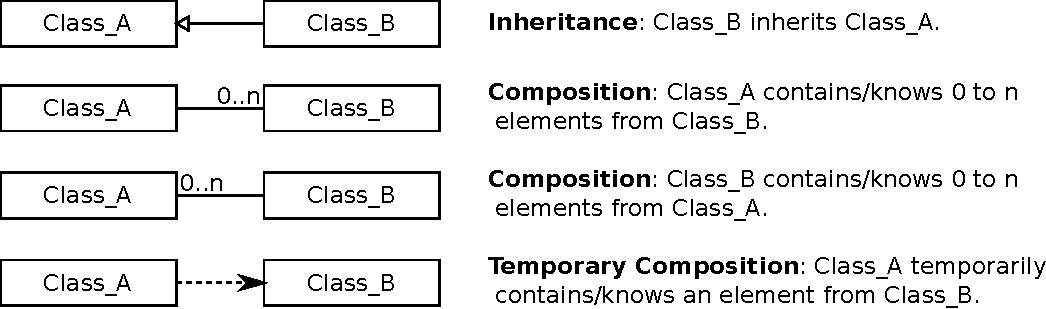
\includegraphics[width=\linewidth]{UML}
  \caption{UML format used.}
\label{fig:UML}
\end{figure}
